\section{Durchführung}
\label{sec:durchfuehrung}

In diesem Abschnitt sollen der Versuchsaufbau,
sowie das Vorgehen der Justierung und der eigentlichen Messung beschrieben werden.


\subsection{Versuchsaufbau}

Für diese Messung wird ein Labordiffraktometer verwendet,
welches eine Röntgenröhre und einen Detektor beinhalten,
die sich um einen Probentisch in der Mitte der Anordnung drehen lassen.
Die hier verwendete Röntgenröhre besitzt eine Kupfer-Anode,
an der eine Spannung von \SI{40}{\kilo\volt} anliegt.
Die entstehende Röntgenstrahlung wird mithilfe eines Göbelspiegels parallelisiert.
Anschließend treffen die Strahlen auf die Probe,
welche sich auf einer Aluminium-Halterung befindet.
Die Intensität der reflektierten Strahlung wird mithilfe eines Detektors gemessen,
welcher sich gegenüber der Röntgenröhre befindet.


\subsection{Justage des Diffraktometers}

Zu Beginn müssen die Position der einfallenden Röntgenstrahlung,
der Probe und des Detektors so justiert werden,
dass der Strahl bestmöglich auf die Probe trifft und reflektiert wird.
Zu diesem Zweck lassen sich die Raum-Positionen der Probe,
sowie die Winkel-Positionen des Detektors und der einfallenden Röntgenstrahlung variieren.
Die Justage beinhaltet verschiedene Scan-Typen,
welche über ein Computerprogramm durchgeführt werden.
Über dieses Programm können auch die Messintervalle und die einzelnen Positionen eingestellt werden.
%wie in \autoref{fig:programm} dargestellt.
%\begin{figure}
%    \centering
%    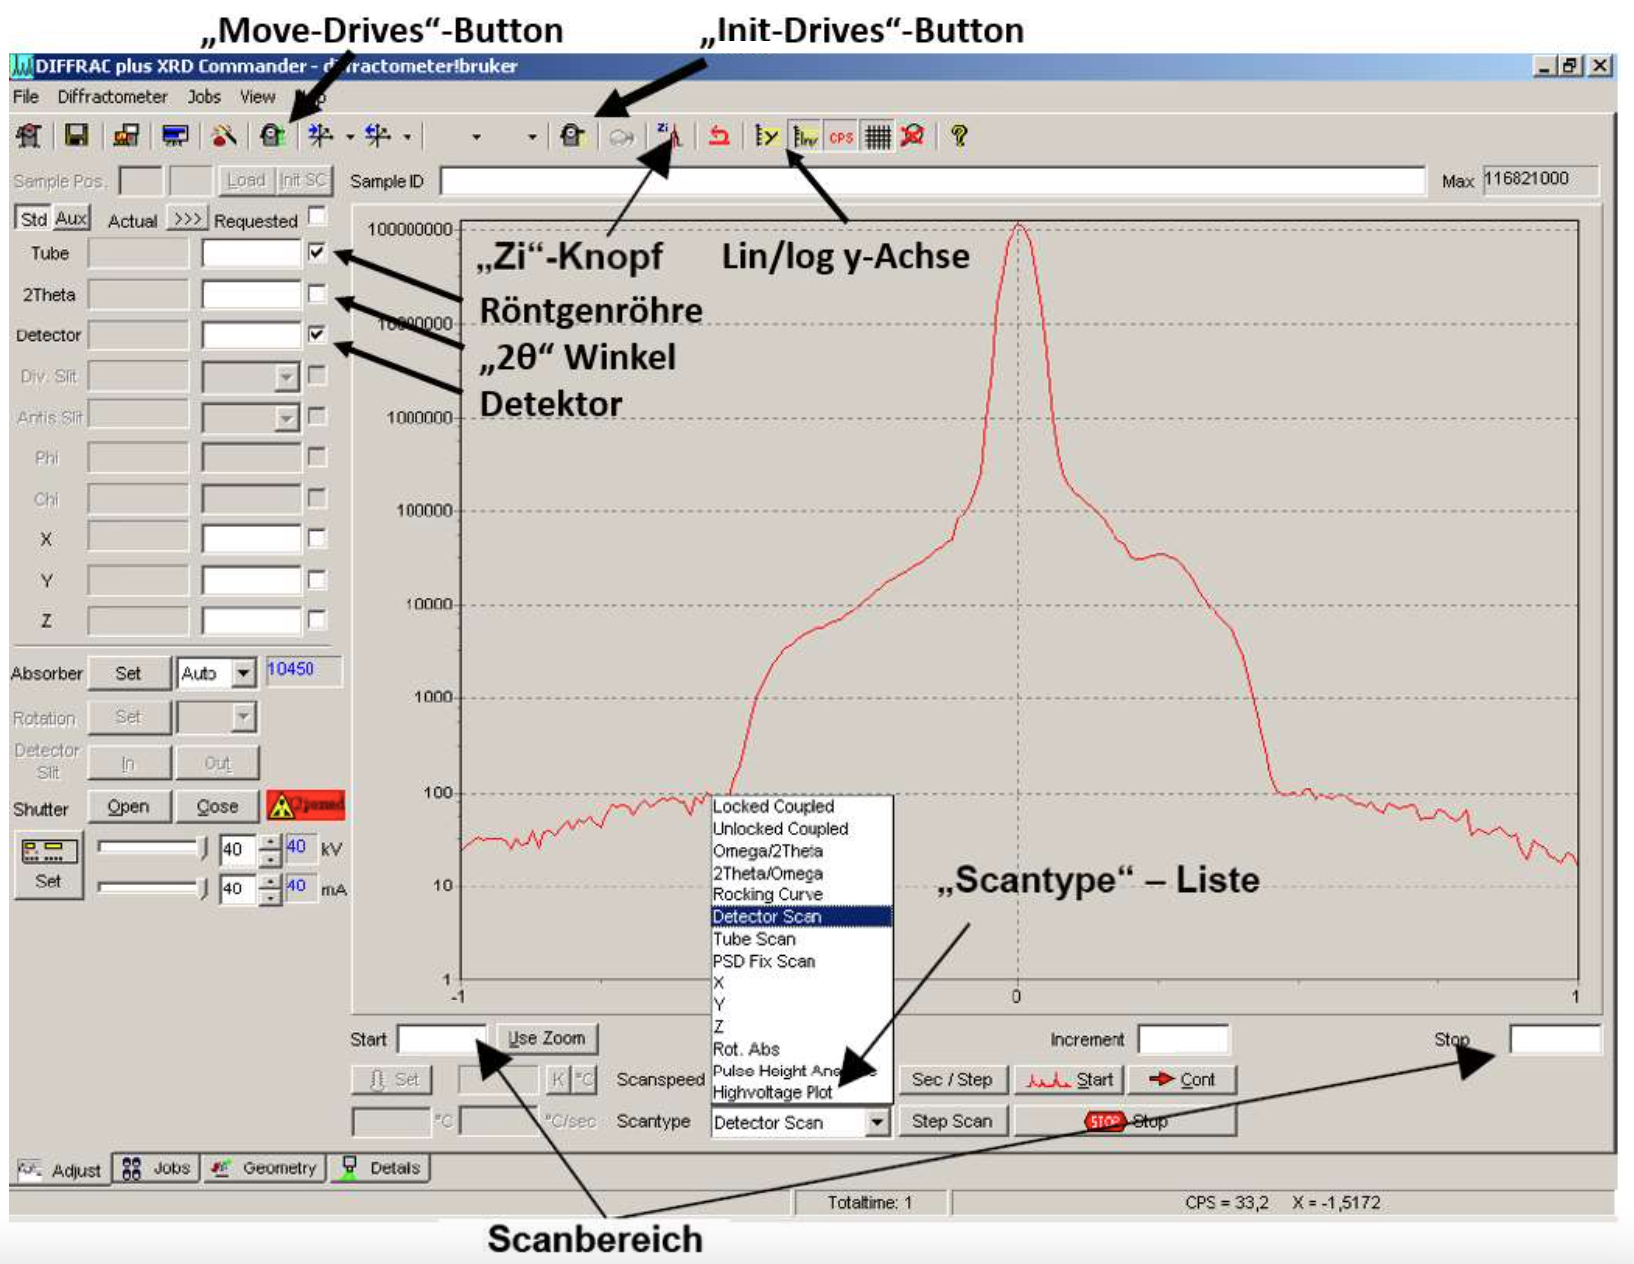
\includegraphics[width=0.5\textwidth]{content/img/Abb_2.png}
%    \caption{Verwendetes Computerprogramm zur Justierung der einzelnen Positionen der Probe,
%    des einfallenden Röntgenstrahls und des Detektors.
%    Es können zudem verschiedene Scan-Typen und Messintervalle ausgewählt werden. \cite{versuchsanleitung}}
%    \label{fig:programm}
%\end{figure}

Bevor mit der eigentlichen Justage begonnen wird,
wird der Absorber auf \emph{AUTO} gestellt,
um den Detektor nicht zu beschädigen.
Anschließend werden alle Positionen auf Null eingestellt.
Bei den jeweiligen Scans wird jeweils eine Messzeit von \SI{1}{\second} ausgewählt.

Nun wird zuerst ein \emph{Detektorscan} durchgeführt,
bei dem die Intensitätsverteilung der Röntgenstrahlung gemessen wird.
Diese sollte,
wie in \autoref{fig:scan} eine Gauß-Verteilung ergeben,
deren Maximum händisch als Null-Position des Detektors eingestellt werden muss.
Dies geschieht über den ZI-Schalter.
Der Messbereich liegt hier zwischen \SIrange{-0.5}{0.5}{\degree} mit einer Schrittweite von \SI{0.02}{\degree}.

Anschließend wird ein \emph{Z-Scan} gestartet,
bei dem die Z-Position der Probe in einem Bereich von \SIrange{-1}{1}{\milli\meter} mit einer Schrittweite von \SI{0.04}{\milli\meter} verschoben wird.
Damit die Probe mittig im Strahl liegt,
muss für die Z-Position ein Wert gewählt werden,
für die die Intensität gerade $I = \sfrac{1}{2} I_\text{max}$ beträgt.
Der Verlauf der Intensität sollte in etwa wie in dem unteren Diagramm in \autoref{fig:scan} dargestellt sein.
\begin{figure}
    \centering
    \begin{subfigure}{0.48\textwidth}
        \centering
        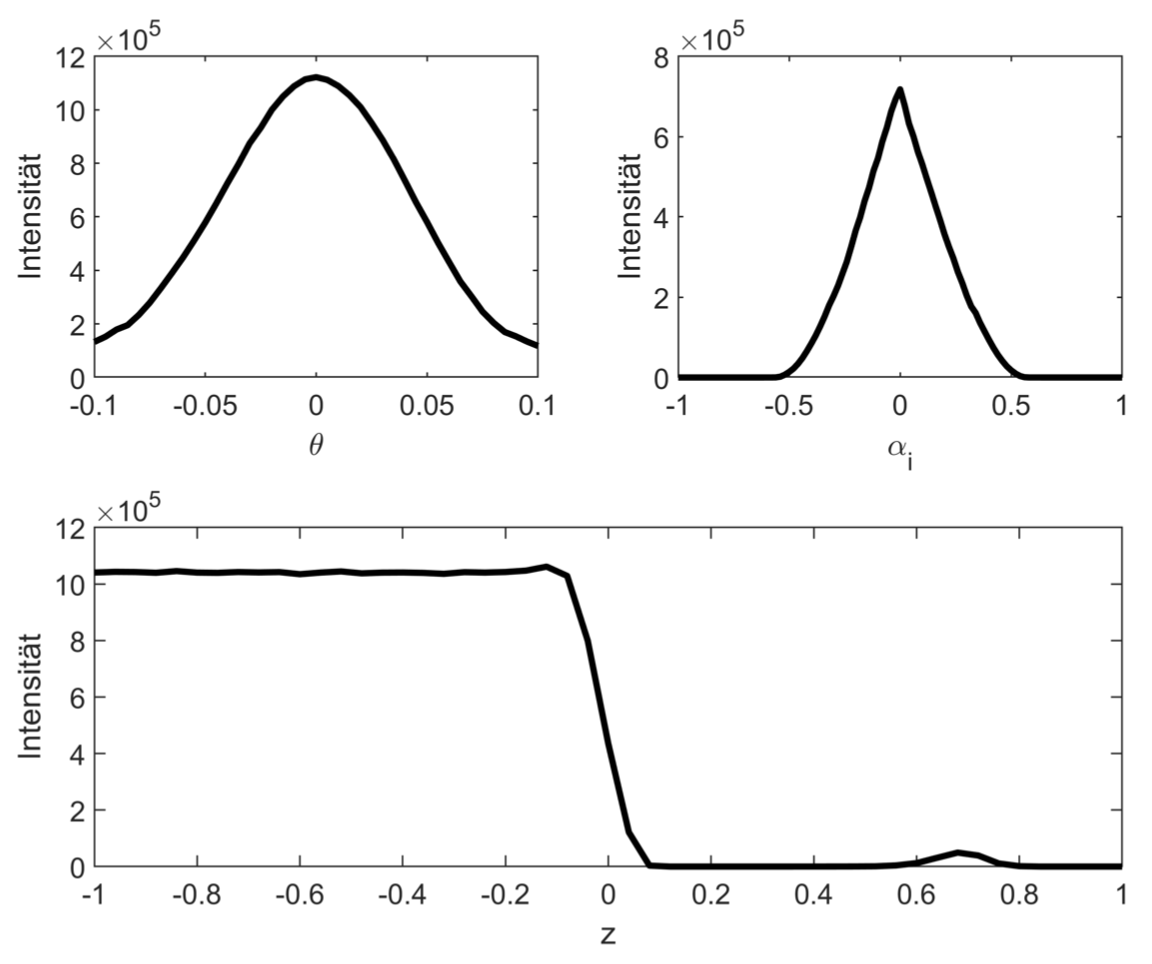
\includegraphics[width=\textwidth]{content/img/Abb_5.png}
        \caption{Intensitätsverteilung beim Detektorscan (oben links),
        Rocking-Scan (oben rechts) und Z-Scan (unten) \cite{versuchsanleitung}.}
        \label{fig:scan}
    \end{subfigure}
    \hfill
    \begin{subfigure}{0.48\textwidth}
        \centering
        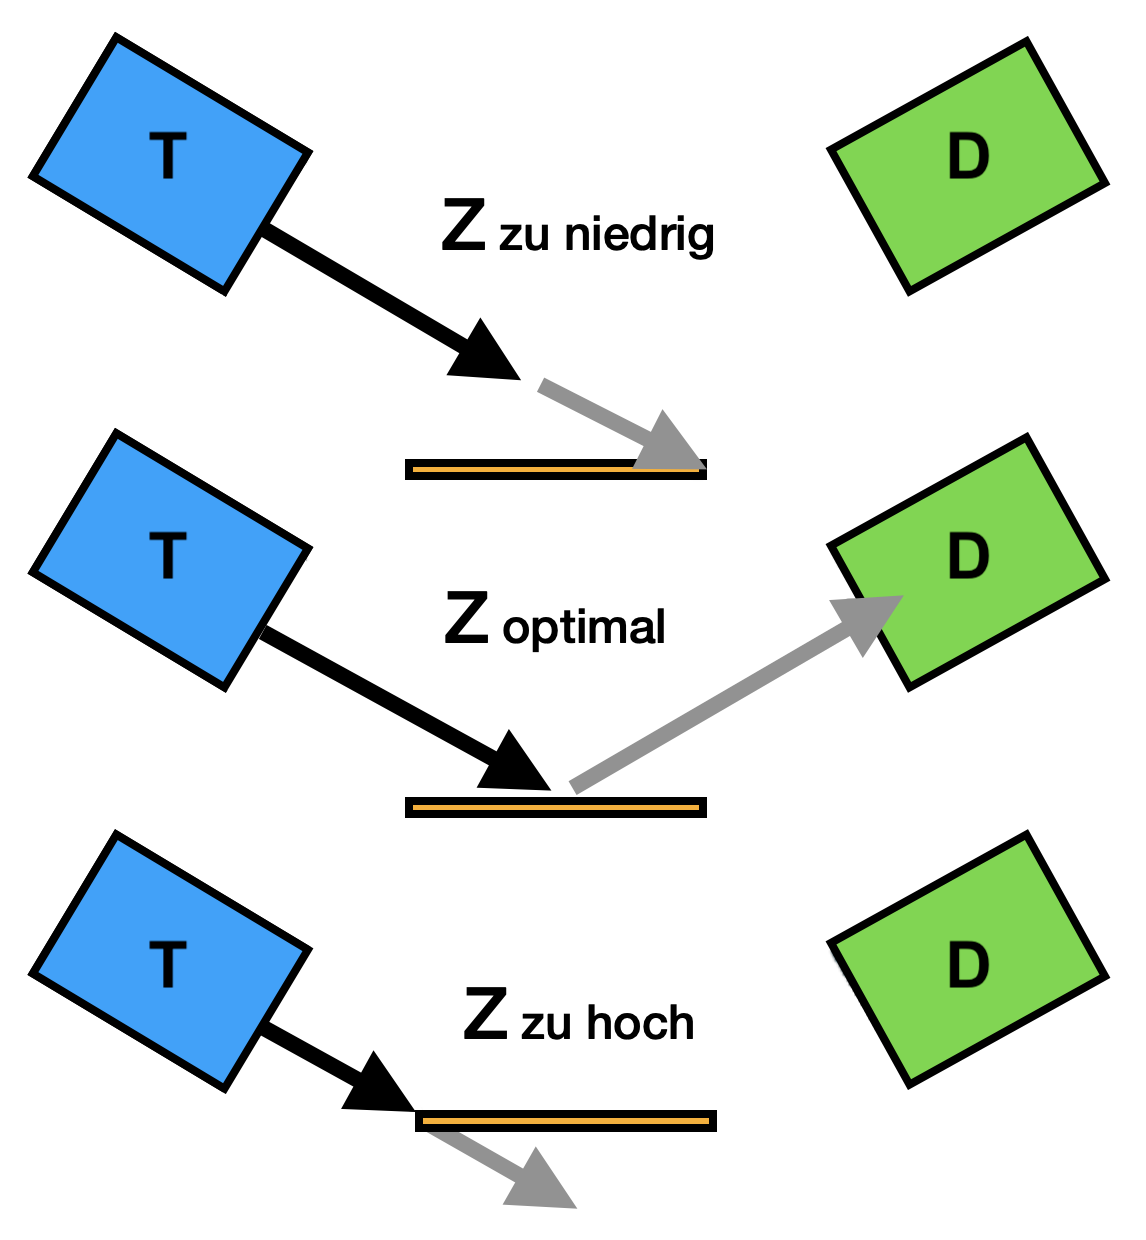
\includegraphics[width=0.65\textwidth]{content/img/Abb_6.png}
        \caption{Verschiedene Z-Positionen der Probe zur einfallenden Röntgenstrahlung und zum Detektor bei einer Winkelsumme von $2\Theta = \SI{0.3}{\degree}$.
        Für eine optimale Reflexion sollte die Probe so liegen,
        dass die Hälfte der maximalen Intensität gemessen wird \cite{versuchsanleitung}.}
        \label{fig:zposition03}
    \end{subfigure}
\end{figure}

Ist der gesuchte Z-Wert eingestellt,
wird ein \emph{X-Scan} in einem Intervall von \SIrange{-20}{20}{\milli\meter} in Schritten von \SI{1}{\milli\meter} durchgeführt,
um die X-Position der Probe einzustellen.
Die Intensitätsverteilung bleibt dabei zunächst konstant,
sinkt auf einen Wert ab,
sobald der Strahl auf die Probe trifft,
und steigt wieder auf den ursprünglichen Wert an,
sobald das Ende der Probe erreicht ist.
Für die X-Position sollte ein Wert gewählt werden,
der möglichst mittig in dem Plateau liegt.

Als Nächstes wird ein \emph{Rocking-Scan} durchgeführt,
um die Y-Koordinate zu bestimmen.
Dabei drehen sich die Röntgenröhre und der Detektor mit konstanter Winkelsumme um die Probe.
Für diesen ersten Rocking-Scan wird eine Winkelsumme von $2 \Theta = \SI{0}{\degree}$ ausgewählt.
Die Intensitätsverteilung sollte einem um Null symmetrischen Dreieck entsprechen,
wie es in \autoref{fig:scan} dargestellt ist.
Weicht die Verteilung davon ab,
muss die Y-Koordinate angepasst werden.
Der Scanbereich läuft hier von \SIrange{-1}{1}{\degree} mit einer Schrittweite von \SI{0.04}{\degree}.

Nun wird ein weiterer \emph{Z-Scan} gestartet,
um die Probe wieder mittig in den Strahlengang zu bringen.
Das Vorgehen bleibt wie zuvor beschrieben.

Um die Justierung weiter zu verbessern,
wird erneut ein \emph{Rocking-Scan} durchgeführt,
wobei die Winkelsumme in diesem Fall $2 \Theta = \SI{0.3}{\degree}$ beträgt.
Es wird ein Messintervall von \SIrange{0}{0.3}{\degree} mit einer Schrittweite von \SI{0.005}{\degree} ausgewählt.
Die Intensitätsverteilung sollte einem um etwa $\Theta = \SI{0.15}{\degree}$ symmetrischen Peak entsprechen,
dessen Maximum mithilfe des ZI-Knopfes manuell auf exakt \SI{0.15}{\degree} verschoben wird.

Abschließend wird mit eingestelltem Winkel der Röntgenröhre und des Detektors ein weiterer \emph{Z-Scan} ausgeführt,
wie in \autoref{fig:zposition03} gezeigt,
wobei die Intensitätsverteilung nun ebenfalls die Form einer Gauß-Verteilung besitzt.
Das Messintervall beträgt hier \SIrange{-0.1}{0.5}{\degree} mit einer Schrittweite von \SI{0.02}{\degree}.
Für den Z-Wert wird das Maximum der Verteilung ausgewählt.


\subsection{Messung der Reflektivität}

Zur Messung der Reflektivität der Röntgenstrahlung wird der Scan-Typ \emph{Omega/2Theta} ausgewählt.
Die Winkelsumme von Röntgenröhre und Detektor sollte wieder $2 \Theta = 0$ betragen.
Es wird ein Intervall von \SIrange{0}{2.5}{\degree} mit einer Schrittweite von \SI{0.005}{\degree} und einer Scanzeit von \SI{5}{\second} eingestellt.

Im Anschluss an diese Messung wird der Detektor um \SI{0.1}{\degree} zum Einfallswinkel verschoben,
um Streuungen herauszufiltern.
Dies wird als \emph{Diffuser Scan} bezeichnet.
Das Messintervall,
sowie die Scanzeit bleiben identisch zur vorherigen Messung.

Abschließend zur Messung werden alle Daten über das Computerprogramm gespeichert.
